\section{Training Stabilizes if a Model Commits to a Rule}
\label{sec:stability}
Why do some runs fail to generalize hierarchically even when trained on hierarchy-inducing data? In this section, we will show that these failures are consequences of training instability; models only stabilize OOD if they commit to a general rule, whether it is the hierarchical or linear rule. Some random seeds fail to stabilize regardless of our training set composition.


\subsection{Instability During Training} 
\label{sec:tv_def}
When training models on both QF and TI tasks, some random seeds lead to highly unstable OOD behavior, with OOD generalization accuracy oscillating during training (see Appendix \ref{appdx:training_instabilty} for example training curves). We measure instability across training time using \textbf{total variation} (TV). Specifically, we checkpoint the model every 2K steps and measure the generalization accuracy $\mathrm{Acc}_t$ at each checkpoint timestep $t \in T$. The total variation is defined as: 
\begin{wrapfigure}[]{r}{0.4\textwidth}
    \centering
    \vspace{5mm}
    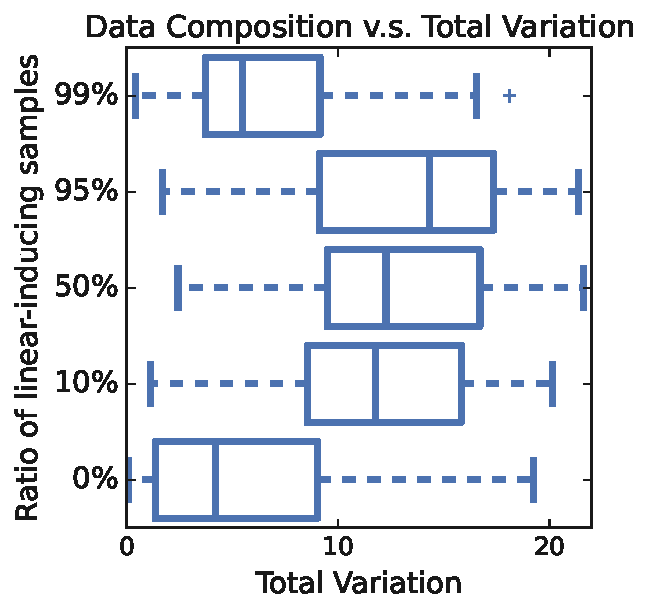
\includegraphics[width=0.85\linewidth]{figures/total_variation_box.pdf}
    \caption{\textbf{Training is unstable when different subsets of data compete.} Balanced mixtures of right-branching and center-embedded sentences have higher total variation than mixtures dominated by one or the other subset.}
    \vspace{-15mm}
    \label{fig:data_drives_inconsistency}
\end{wrapfigure}
\begin{align}
    \text{Total Variation (TV)} = 
    \frac{1}{|T|} \sum_{t \in T} 
    \left| \mathrm{Acc}_t - \mathrm{Acc}_{t-1} \right|
\end{align}

\subsection{Training Stability Ties to Rule Commitment}
\label{sec:intra_inter}

We now demonstrate that stable OOD behavior is associated with rule commitment. We construct QF training datasets with different proportions of hierarchy-inducing (i.e., center-embedded) and linearity-inducing (i.e., right-branching) declaration examples, while keeping all question examples from the original training set. Further details on the dataset can be found in Appendix~\ref{sec:simple_mixin}.


Figure \ref{fig:data_drives_inconsistency} shows the relationship between data homogeneity and training stability. When the training data is dominated by either linearity-inducing  (99\% linear) or hierarchy-inducing  (0\% linear) examples, more random seeds lead to stable OOD curves. When the training data is a heterogeneous mix instead, potential rules compete, leading to a higher proportion of unstable training runs.

By controlling for training instability, we reveal that generalization behavior is clustered and highly bimodal across random seeds. As shown in Figure \ref{fig:intra_inter_variance}, regardless of the data mix, the final generalization accuracy for all stable models is either $100\%$ or $0\%$---that is, stable models always commit to a systematic rule. 
While either rule can be implemented by a stable model, training data composition determines how likely a run is to stabilize in any rule and whether that rule is likely to be hierarchical or linear. 
Interestingly, when the data is heterogeneous (e.g., 10\% of examples are linearity-inducing right-branching sequences), the final generalization accuracy for stable runs is bimodally distributed, clustering around $100\%$ or $0\%$. 
 In fact, the horseshoe-shaped curves in Figure \ref{fig:intra_inter_variance} illustrate that the less stable a training run is, the less systematic the model tends to be in its OOD rules. 

\begin{figure}[t!]
    \centering
    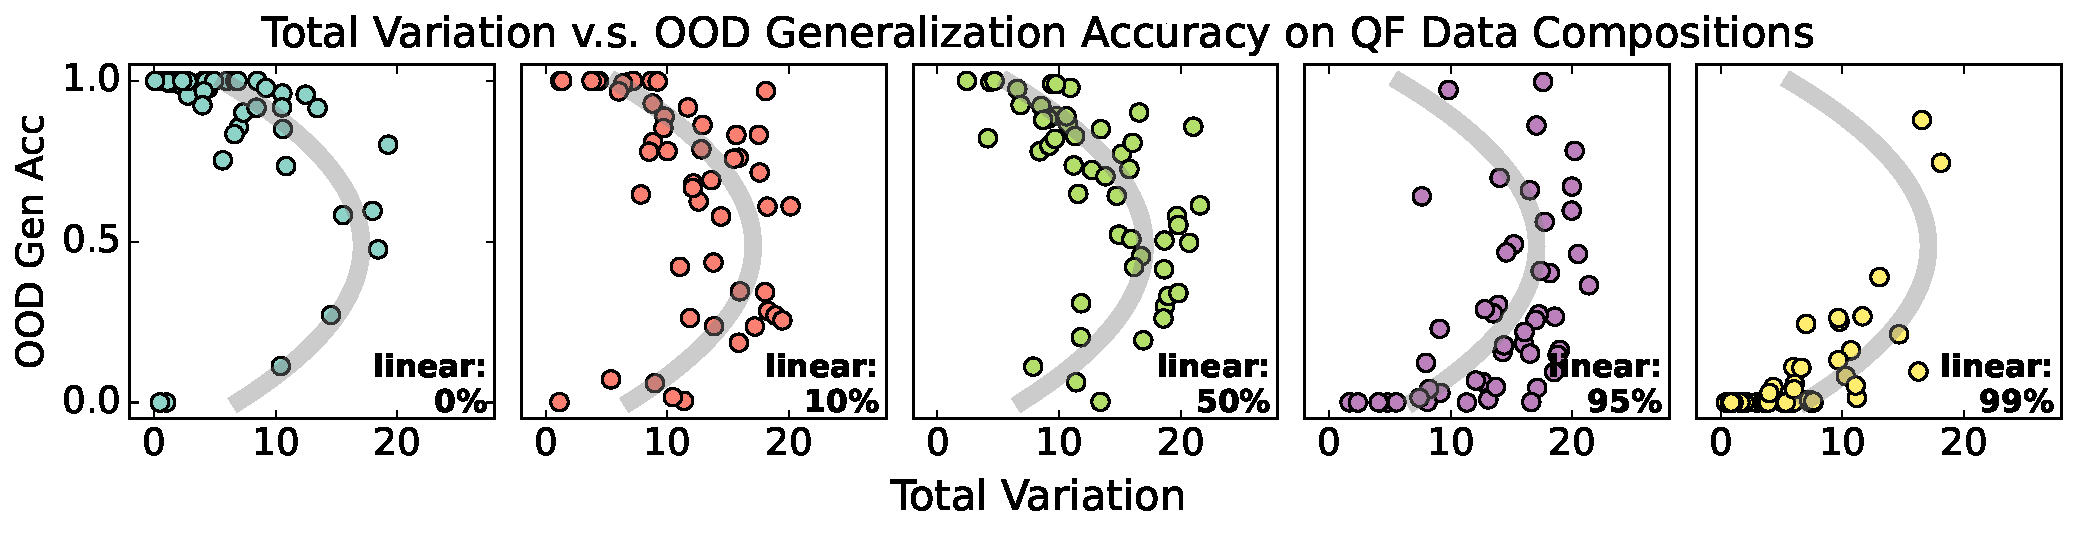
\includegraphics[width=1.0\linewidth]{figures/intra_inter_inconsistency_D270.pdf}
    \caption{\textbf{Training stability vs. final generalization accuracy for QF task.} OOD behavior stabilizes during training if a model commits to a general rule. By mixing data that induces the linear and hierarchical rules, we can create conditions that allow models to stabilize in either rule. ``Linear" denotes the proportion of linearity-inducing declarations in the data. 
    Grey line indicates the smoothed average curve across all five datasets.
    }
    \label{fig:intra_inter_variance}
    % \vspace{-5px}
\end{figure}

In summary, with heterogeneous training data, competition between rules leads to more unstable training runs. Even with heterogeneous data mixes, however, some runs can still stabilize if they  commit to one of the competing rules. Therefore, heterogeneous data also leads models to cluster into bimodally distributed OOD generalization accuracies, reflecting the distinct basins observed by \citet{Juneja2022-hj} in text classification.
Appendix \ref{appdx:tense_tv} presents similar findings for the TI task.

